\documentclass[a4paper,11pt]{article}
\usepackage[utf8]{inputenc}
\usepackage[T1]{fontenc}
\usepackage[margin=2cm]{geometry}
\usepackage{graphicx}
\graphicspath{{./}{visual_abstract/}}
\usepackage{hyperref}
\usepackage{parskip}
\usepackage{titlesec}
\usepackage{xcolor}
\usepackage{booktabs}
\usepackage{microtype}
\usepackage{caption}

\definecolor{uiablue}{RGB}{0,84,166}
\definecolor{darkgrey}{RGB}{80,80,80}

\hypersetup{colorlinks=true, urlcolor=uiablue, linkcolor=uiablue}

\titleformat{\section}{\large\bfseries\color{uiablue}}{}{0em}{}[\titlerule]

\begin{document}

% ── Header ───────────────────────────────────────────────────────────────────
\begin{center}
{\LARGE\bfseries\color{uiablue}
NAS-Guided FEM-Anchored PINNs\\[4pt]
for Transient Heat Transfer Simulation}

\vspace{4pt}
{\large\color{darkgrey}
Step Optimization in Thermal Simulation Using\\
Selective Finite Element Method Step Skipping}

\vspace{10pt}
\begin{tabular}{ll}
\textbf{Author:}     & Ömer Çetinkaya \\
\textbf{Supervisor:} & Prof.\ Turgay Celik \\
\textbf{Institution:} & University of Agder (UiA), Norway \\
\textbf{Year:}       & 2026 \\
\end{tabular}
\end{center}

\vspace{6pt}
\hrule height 1.5pt
\vspace{10pt}

% ── Abstract ─────────────────────────────────────────────────────────────────
\section*{Abstract}

In this thesis, we developed a Finite Element Method (FEM)-anchored
Physics-Informed Neural Network (PINN) framework for transient water-quenching
simulation of A356 aluminium.
We based the study on the industrial quenching scenario of Mortensen et al.\ (2026).
Our central question was: how many FEM solver calls can be replaced by PINN
predictions while keeping the temperature error within engineering limits?

We adopted Multi-Step Window Prediction (MSWP) as the core strategy.
The FEM solver provides anchor temperature fields at selected time steps; the
PINN predicts the field between consecutive anchors.
The skip factor $k$ controls the anchor spacing.
We compared three Neural Architecture Search (NAS)-selected architectures:
Bayesian/TPE ($5{\times}151$, ReLU), NSGA-II ($3{\times}153$, tanh), and
NSGA-III ($3{\times}75$, tanh).
We conducted experiments across ten unique benchmark geometries in two studies.
The canonical study covers eight domains: three 2D, four 3D, and the Thermal Fin,
originally a 2D steady-state RBniCS benchmark that we extended to a 3D
transient quenching scenario.
A complementary adaptive-$k$ study added Square and Flower as two new 2D geometries.

On the adaptive-$k$ study, we found 83--85\% FEM saving with mean absolute
error (MAE) below $2.5\,^\circ$C across all architectures.
On the canonical 2D domains with fixed $k$, Bayesian/TPE stayed below
$5\,^\circ$C through $k=3$ on all three domains.
On the 3D domains, Bayesian/TPE remained acceptable at $k=5$ with MAE below
$14\,^\circ$C.
On the Thermal Fin, Bayesian/TPE with Fourier embedding reached $k=5$ at
$12.55\,^\circ$C (ten-seed mean).
NSGA-II and NSGA-III held through $k=4$.
We demonstrated that FEM-anchored PINNs can reproduce transient quenching
fields with 65--85\% fewer solver calls within practical engineering accuracy.

\noindent\textbf{Keywords}\quad Physics-Informed Neural Networks, Neural Architecture Search, Finite Element Method, Transient Heat Transfer, Water Quenching, Multi-Step Window Prediction, Adaptive Skip-Factor Scheduling, FEM-Anchored Surrogate Modelling, Fourier Feature Embeddings, Thermal Fin Benchmark, A356 Aluminium.

\vspace{10pt}

% ── Visual Abstract ───────────────────────────────────────────────────────────
\section*{Visual Abstract}

\begin{figure}[h!]
\centering
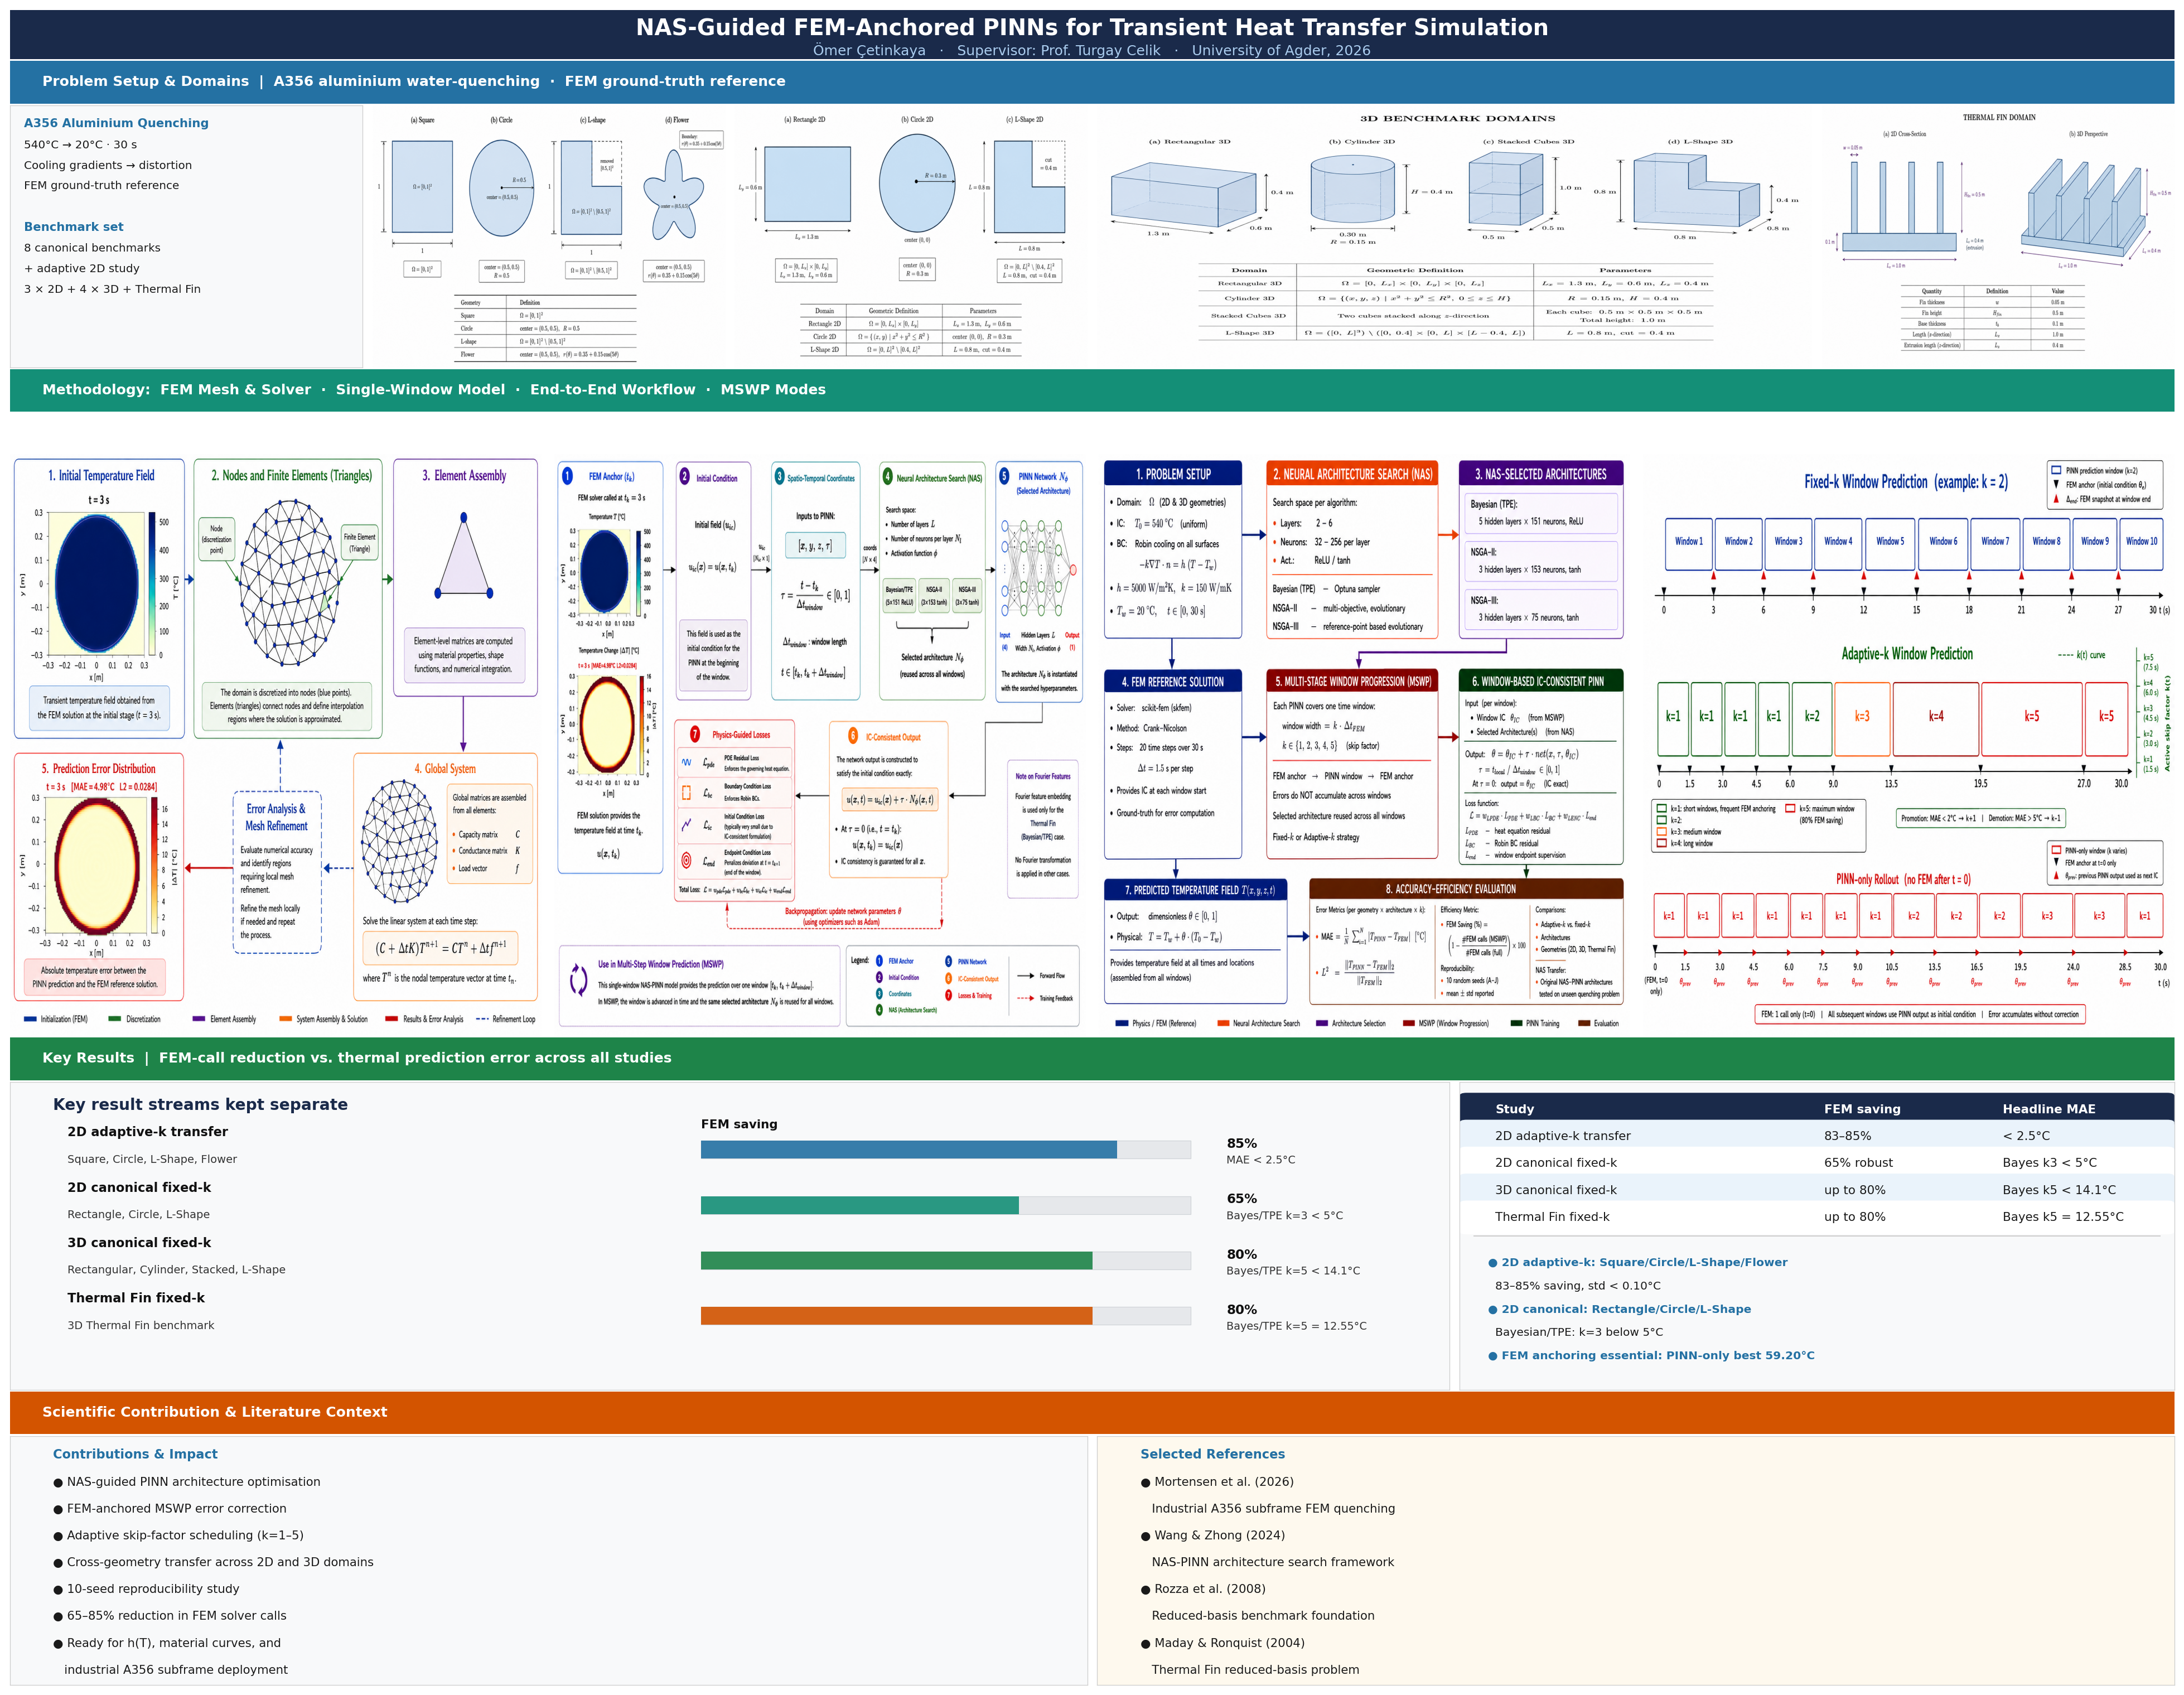
\includegraphics[width=\textwidth]{visual_abstract.png}
\caption*{Visual summary of the thesis. The top row defines the A356
water-quenching problem and benchmark geometries; the middle row summarises the
FEM reference solver, NAS-PINN framework, and MSWP strategy; the lower rows
highlight the main accuracy--efficiency results, scientific contributions, and
application impact.}
\end{figure}

\vspace{8pt}
\section*{Selected References}
\small
Mortensen et al. (2026), ``Mitigating distortions in cast automotive subframes.''
Wang and Zhong (2024), ``NAS-PINN: Neural architecture search-guided physics-informed neural network.''
Rozza et al. (2008) and Maday and Ronquist (2004), reduced-basis/Thermal Fin benchmark references.

\end{document}
